So far I have discussed the formalisation of \kl{CN}, the formalistaion and
implementation of its memory model, \kl{CN-VIP}. In both those sections,
guiding design choices and implementation decisions at each stage was the need
to strike a balance of expressiveness, performance and ergonomics,
fundamentally motivated by designing a \emph{capable} verification tool. Not
only that, at several stages, the theory was able to inform or clarify
implementation related issues, such as the complexity of adding new features,
lifting existing restrictions, or substantially improving performance.

In this part, I will take a step back and focus more on what it takes to build
a \emph{usable} verification tool. Though not as theoretically intruiging or
elegant as some of the material in the previous chapter, this is where just as
much, if not more, of the difficulty lies in achieving \kl{CN}'s goal of being
maintainable by kernel hackers (\cref{sec:cn-goals}).

It start with the source repository for any mature C project, such ask
\kl{pKVM}. It intentionally lives in the Linux kernel, indeed in many respects
this is an advantage. It is an unignorable reminder that C in the real word
however does not come neatly packaged up into isolated files of ISO grammar
conforming translations units. Aside from the myriad extensions that it relies
on, as well as non-ISO conforming C features, the inclusion chain of one file a
few hundred lines long can stretch \emph{eleven} directories up and total
around 65,000 lines of C after preprocessing. Mature industrial projects like
GCC and Clang have spent years optimising their front-ends to deal with this
complexity at speed, which creates a large gap between it, and robust,
empirically validated, but ultimately academic tools such as \kl{Cerberus}.

Thankfully, there is an alternative to simply adding features to the
\kl{Cerberus} frontend until it can handle a substantial number of GCC and
Clang fragments. In our experience, the set of features used by a particular
directory of files, such as the \kl{pKVM} project are relatively small, and can
be manually extracted by copying files, commenting out unused features, and
flattening directory hierarchies. Whilst this is possible, it is tedious, slow,
error prone and extremely time consuming, taking days to perform by hand,
making it very difficult to update once code is updated. Doing so trades-off
implementation and intellectual effort for grunt work and drudgery, which is a
step in the right direction, albeit no more practicable.

Faced with this, and the awareness of tools such as clang-format, which can
format complex projects of C++ code, including macros, and other Clang based
tools for linting and refactoring, I developed a tool which could automate the
aforemention drudgery. Analagous to tree-shaking for JIT-compiled interpreted
languages, I call the method \intro{tree-carving}, which given a root file in a
repository, extracts out the files in the transitive dependency of that root,
and comments out anything not used.\sidenote{Such a strategy works for most
sensibly formatted code with each top-level declaration on its own line. For
code which does not fit this, input validation will reject the program rather
than produce erroneous output.} It comments out code to preserve line numbers,
and works with macros too. Since \kl{CN} specifications are comments too, and
could get lost inside other comments, I also wrote a comment simplifier to undo
such nested comments.

Even with reasonable input, the challenges continue. One of the early
challenges \kl{CN} faced was that of allocation for function arguments. Though
intuitively, a programmer might model allocations for parameters as being
created by the \emph{callee}, early versions of \kl{CN} relied on
\kl{Cerberus}' elaboration allocating storage for function arguments at the
\emph{caller}, per callsite. This significantly degraded the experience of
writing specifications and proofs because the programmer had to specify that
functions did not mutate arguments at the callsite. Kayvan Memarinan fixed this
by creating a parallel mode of elaboration to support the more intuitive model.

Influenced by \kl{Cerberus}'s decision to model C integers as unbounded with
constraints, \kl{CN} originally adopted a similar design, and used to verify
the \kl{pKVM}'s buddy allocator, as mentioned in \sidetextcite{pulte2023cn}.
However, this soon became cumbersome due to the use for frequent bit
manipualation idioms in \kl{pKVM}'s page table walker, because expressing these
idioms on integers then required the frequent use of lemmas to handle the
(undecidable) non-linear arithmetic. This prompted an overhaul of \kl{CN} to
work with bit vectors as its fundamental integer type.

My contributions to this thread began as I attempted to update the buddy
allocator to handle a very early version of \kl{VIP}, which coincided with the
move to bitvectors, \emph{and} a change in the inference scheme. Alongside
this, this was my first serious use of \kl{CN} and separation logic, and I did
not have the benefit of the helpful \kl{CN tutorial} to serve as less steep
cliff to ascend. To top it all off, the underlying code of the buddy allocator
had been updated, unbeknownst to anyone at the time (we did not have
performance benchmarking) \kl{CN} became dramatically slower, and at the time
had no ability to track source location information across the majority of its
pipeline. Whilst the attempt seems foolish and doomed from the start, it
clarified a few things we needed to improve upon.
\begin{itemize}
    \item Source location information.
    \item Regression testing.
    \item Peformance benchmarking.
    \item Switchable major transitions.
    \item A tutorial and worked examples.
    \item Upating proofs one aspect at a time.
\end{itemize}

As result of this failed attempt, I came to appreciate all the above. I ended
up spending about one month plumbing through source location information
through out the core datatype in \kl{CN}, as well as fixing the lexer and
parser to be more robust and have extensible error messages.

I also identified a particularly difficult challenge which any verification
tool based on an internal representation needs to deal with is relating errors
back to the source code user wrote. This is particularly evident with SMT
counter-examples which are not minimal, consistent, nor easy to translate back
to the source. Aside from this, even in the absence of \kl{VIP} related
performance issues, \kl{CN} is still about an order of magnitude slower than we
would like it to be, though the causes of this are not clear, the plan of being
able to rely on performant SMT solvers with decidable queries has not paid off
quite as well as we would have liked.

\chapter{Tree-carving: Taming C Respositories}\label{chap:tree-carver}

\margintoc{}

In this chapter, I will explain why we need a tree-carver for C repositories,
by referring to the mounting challenges we were facing scaling \kl{Cerberus} to
handle large repositories. After that, I will explain the features of C which
make this a particularly challenging endeavour, mostly centred on macros and
the C preprocessor. I will also explain why it is very desirable to \emph{not}
input preprocessed C code into verification tools such as \kl{CN} (constants,
and column information). Lastly, I will show how, extending prior work
significantly, I built a Clang-based tool which meets almost all the
requirements we sought, enough to not be the primary bottleneck to verifying
code in large projects anymore. Laslty, I will explain the limitations of the
current approach (struct fields, cross-translation-unit carving), and ways this
may be remedied in the future.

\section{Need for tree-carving}

I will use the \kl{pKVM} page-table code as the motivation for the chapter.
It lives in the folder arch/arm64/kvm/hyp/pgtable.c, and consists of some simple
functions like the one below, for converting a page-table entry to a physical
address.

% c-tree-carve -r kvm_pgtable_hyp_map arch/arm64/kvm/hyp/pgtable.c -n 0

\cfile[fontsize=\footnotesize,breaklines,lastline=7]{code/pgtable.c}

It also includes more complicated functions such the one below which uses function
pointers, arguments, and flags in a struct to effectively create a closure, with
which to call a parametric page-table walking function.

\cfile[fontsize=\footnotesize,breaklines,firstline=9]{code/pgtable.c}

This code is not suitable to be input to \kl{Cerberus} because of the fact
is uses features it does not support. However, these features are not at
all obvious from just looking at the code; one would expect the only features
used are macro constants, and regular C declarations for types and functions.

Let us start with \cinline{KVM_PTE_ADDR_MASK}. This is defined using another
macro, \cinline{GENMASK}.

\cfile[fontsize=\footnotesize,breaklines,lastline=2]{code/kvm_pte_addr_mask.c}

In turn, \cinline{GENMASK} is defined using two macros, in separate file. The
second of these, \cinline{__GENMASK} is the one which defines the constant in
the expected way as a bit-shifting expression. However, the first,
\cinline{GENMASK_INPUT_CHECK}, relies on two other macros
\cinline{BUILD_BUG_ON_ZERO} and \cinline{__isconstexpr} and a compiler
intrinsic, \cinline{__builtin_choose_expr}.

\cfile[fontsize=\footnotesize,breaklines,firstline=3,lastline=14]{code/kvm_pte_addr_mask.c}

The \cinline{__isconstexpr} macro is defined in yet another file. I do not
understand how this works, and in any case, \kl{Cerberus} rejects it.

\cfile[fontsize=\footnotesize,breaklines,firstline=16,lastline=23]{code/kvm_pte_addr_mask.c}

The GCC built-in \cinline{__builtin_choose_expr} happens to take to expressions
as its arguments, but in general this is not the case. For example, the
\cinline[breaklines]{__builtin_types_compatible_p} takes two \emph{types} as
its argument. Such built-ins require editing the parser and elaboration to
support, and cannot be abstracted easily.

Lastly, \cinline{BUILD_BUG_ON_ZERO} uses the expression to try to construct an
anonymous struct with a bit-field of that size, since 0-width bit-fields are
not allowed, this will trigger a build error. Bit-fields are not supported by
\kl{Cerberus} either.

\cfile[fontsize=\footnotesize,breaklines,firstline=25,lastline=26]{code/kvm_pte_addr_mask.c}

Whilst the use of robust compile-time checks is laudable, the features
involved, the trail of dependencies of macros across different files and the
lack of \kl{Cerberus} front-end support for them makes them a non-starter to
even ignore when verifying code with \kl{CN}.

Remember, this is the thread that unravelled by inspecting just
\cinline{KVM_PTE_ADDR_MASK}. In this case, there is a simple workaround
(redefine the \cinline{GENMASK} macro to not do any compile time checks). In
general, it is not is not possible to tell if a particular part of the code is
ignorable, or used by the code one wishes to verify. This is particularly
inconvenient because it then becomes difficult to distinguish whether a
particular feature is unavoidable and worth implementing in \kl{Cerberus}, or
just an incidental block to parsing, but otherwise safely ignored.

In other words, \emph{if parsing fails on a file, we are forced to implement
the construct in the parser, regardless of whether or not is is used later,}
which is not an efficient use of engineering capacity. As seen above, Linux
headers and macros frequently contain such constructs, so the issue persists
even after preprocessing.

\section{Challenging preprocessor and C features}

One may think that preprocessing will sidestep this issue, because unused
macros (and accompanying unsupported features) will not be pasted into the
code.

Unfortunately, whilst this does avoid the myriad problems of doing dependency
analysis on macros, it comes with trade-offs. Take the \cinline{GENMASK} macro
above. If expanded fully into each use site, the code to verify would be
littered with unsupported features. The structure of the macros and its
dependency, (the fact that there is one part which is a compile-time check, and
another which computes the expression we care about) would be lost, making it
harder to spot what to redefine and where for the purposes of proof.

Preprocessing would also corrupt source location information for
columns.\sidenote{Line directives keep the line information accurate, and
comments can be preserved with the right options} Whilst this is already lost
by the \kl{Cerberus} front-end, it would make it irrecoverable if \kl{Cerberus}
were to upgrade its
lexer.\sidenote{\href{https://github.com/rems-project/cerberus/issues/393}{cerberus\#393}}

Preprocessing will also flatten the directory structure on the original
repository, making it more difficult to relate any output back to the code it
came from. Initially, we assumed that this sort of dependency analysis would be
quite expensive, so the idea was that a user would run the carving once,
annotate the carved code, and then merge the changes back into the source
repository, for which point preserving file structure may be
helpful.\sidenote{The alternative would be to create patches based on the line
directives in the single preprocessed files.}

However, analysing a non-preprocessed file is also fraught with difficulty.
Unfortunately, macros are not simply `find-and-replace' abstractions, but can
support conditionals, defining, un-defining and re-defining, as well as be
constructed dynamically with token-pasting. Macros are not stored as part of
the abstract syntax tree and so whether or not it was possible to recover
dependency information from them was an open question.

Aside from the preprocessor, C features such as forward declarations, also make
dependency analysis challenging. For example, a struct can be forward-declared,
code can mention or manipulate pointers to it (but not mention its fields), and
only later do the fields need to be defined. Struct and union fields, typedefs,
function names, types of function locals, arguments and returns, enums and
their initialisers, and array size expressions all form part of the dependency
chain.

Lastly, on a practical level, C files, with all their includes, tend to be
quite large, with examples from \kl{pKVM} easily reaching tens of thousands of
lines with only a standard set of includes. \kl{Cerberus} has typically been
used with much smaller files, and so using it to parse, analyse and ignore the
relevant parts of a C program is not feasible either (on top of the
preprocessing issues mentioned earlier).

\section{Implementation}

As I mentioned earlier, the existence of tools such as clang-format, which
handle formatting code in the presence of macros, and other Clang based tools
for linting and refactoring, led me to suspect it may be possible to build such
a tool using Clang.

The advantages of this would be excellent performance and compatibility with
existing C code, given the amount of investment placed in these tools. Clang
also gives good error messages in the presence of macros, including presenting
how an error inside multiple chained ones presents itself, which indicated that
dependency analysis on macros may be possible.

I owe a large debt to
\href{https://github.com/logicmachine/cpp-simplifier}{logicmachine/cpp-simplifier}.
The tool describes itself as a `C++ source simplifier for competitive programming',
which `expands double-quoted inclusions and removes unused declarations'.
This provide a very useful skeleton and an introduction to Clang's APIs, which
enabled me to modify it in the following ways.
\begin{itemize}
    \item Add C constructs required for kvm\_pgtable\_walk in pgtable.c code.
    \item Support compilation databases.
    \item Support multiple, user-defined root functions.
    \item Retain and reproduce the directory structure.
    \item Support macro dependencies.
    \item Comment out code instead of deleting it.
    \item Simplify comments/recover CN annotations.
    \item Retain all includes.
    \item Validate input for top-level declarations.
\end{itemize}

The tree-carver tool I wrote is called `c-tree-carve'. It is actually two tools
in a trench coat, a `clang-tree-carve.exe' written in C++ for interfacing with
Clang's APIs, and a `comment simplifier' written in OCaml, to recover CN
annotations from line comment after the first tool has run.

At the very least, c-tree-carve requires a compilation database (a
compile\_commands.json file) and a source file named within that database. If
the file is mentioned more than once within the database, then the tool
requires the user to disambiguate which command they intend to run the tool
with. This is important because the options in a command can affect the macros
enabled, their values, the paths in which headers are searched, and the
warnings emitted by the Clang front-end. If no root functions are specified,
the tool uses all the functions declared in the file as roots, otherwise only
the selected roots are used. There is also an optional debug flag which will
trace out the declarations and macros traversed, with their source locations
and their dependencies.

With these options, tree carver sets up a ClangTool instance, which is
essentially an invocation to clang as a user may given on the command line. The
invocation is the combination of the command selected from the compilation
database, plus an extra directive to Clang to store a detailed preprocessing
record, which is necessary to analyse macro dependencies later. To run the
invocation, the ClangTool is also given an instance of FrontendActionFactory.
This is where I override the appropriate methods to ultimately produce a map
from file names to a vector of bools, one for each line in the file to mark it
as present or absent. With that map, it is easy to output, in a new temporary
directory, the source files but with the all but the relevant lines commented
out.

\inputminted[breaklines,fontsize=\footnotesize]{cpp}{code/simplifier.cpp}

The FrontendActionFactory creates an instance of an ASTFrontendAction, in which
is the method I override. It adds a callback to the preprocessor to record
\emph{all} macro expansions when the preprocessor is run. To run the
preprocessor, validate the top-level declarations, traverse and mark each
top-level declaration, requires execute the action on the super object, which
in turn has one more overridden method. After that, with the preprocessing
record, it is possible to find all macro expansions within a given source range
(that of all declarations), and mark all macros and their dependencies as used.

\inputminted[breaklines,fontsize=\footnotesize,lastline=35]{cpp}{code/reachability_analyzer.cpp}

The overridden method in the super object is a handler for the translation unit
as a whole, which takes as its sole argument a reference to an immutable
ASTContext. This simply validates the top-level declarations, traverses the
declarations, adds in any forward declarations required, and then marks the
source ranges for all the declarations as kept lines. The code for traversing
and marking is similar, but represent slightly different concerns and are
currently separated to take into account the correction for forward
declarations. Since performance has not been an issue in practice, the
increased readability and maintainability has been worth the separation.

\inputminted[breaklines,fontsize=\footnotesize,firstline=37]{cpp}{code/reachability_analyzer.cpp}

I shall now describe, at a high level, how I analysed dependencies for macros.
As far as I am aware, this aspect of the tool is especially novel and difficult
to reproduce with other approaches short of implementing a custom preprocessor.
The first step is to accurately capture the source range for macro definitions,
because these can space multiple lines, and the default source ranges for macro
definitions do not capture the range one would expect.\sidenote{The range ends
\emph{before} the start of the last token, rather than including the end of
it.} Doing so is straightforward with a overridden method to handle each macro
as it is defined. Note that the data is indexed not by the macro name, but by
its definition range, which is guaranteed to be unique.

\inputminted[breaklines,fontsize=\footnotesize,lastline=19]{cpp}{code/reachability_analyzer.hpp}

The next step is to record \emph{every macro expansion}. This is again done
with an overridden method, and most elegantly, does not rely on pre-empting or
understanding when and how each macro is expanded, only that it is, and that
its replacement token stream is available. Each time the method is invoked is
either with an outer/top-level macro, or a macro that is inside the expansion
of the most recent outer/top-level macro. In the first case, the definition
range of the outer/top-level macro is recorded. Remember that the definition
range of a macro is a way of uniquely identifying it. In the second case, the
macro is being expanded \emph{inside} the outer/top-level macros. So I record
the fact that (the definition range of) the outer depends on (the definition
range of) the expanded one. The for-loop is only there to calculate
the nesting depth of the dependency for pretty-printing, which is not relevant
for the \emph{transitive} dependency structure being computed.

\inputminted[breaklines,fontsize=\footnotesize,firstline=21]{cpp}{code/reachability_analyzer.hpp}

With this information, the only remaining step is figuring out which macros are
used inside a given declaration. Fortunately, there is a
`getPreprocessedEntitiesInRange(SourceRange)' method inside the % chktex 36
PreprocessingRecord class, which allows one to take a declaration, query its
source range, and then get an iterator of all the preprocessing entities in it,
including macro expansions.

It is not however enough to stop here, because at this stage, although the
resulting file is a valid C program with all unnecessary lines commented out
(including unused headers, and unused fields), reducing thousands of lines of C
to hundreds, the empty and commented lines in between top-level declarations,
which may contain CN declarations, are also commented out.

\inputminted[breaklines,fontsize=\footnotesize]{cpp}{code/clang_tree_carve.cpp}

In this form, \kl{CN} cannot recognise them, and so they need to be recovered.
The code to achieve this is, perhaps surprisingly, an ocamllex program, which
encodes (at a first approximation) a finite state machine
(\cref{fig:comment-simp-fsm}). The implementation is complicated slightly by
the fact that in C/C++, lines terminating with a backslash may be spliced
together with the next line, and so a line-comment may actually extend over
multiple lines. Whilst this is not a common use of line splicing, it is heavily
used in macro definitions. The result is the comments are simplified but things
which are commented out stay commented out.

\begin{figure*}[tp]
\begin{center}
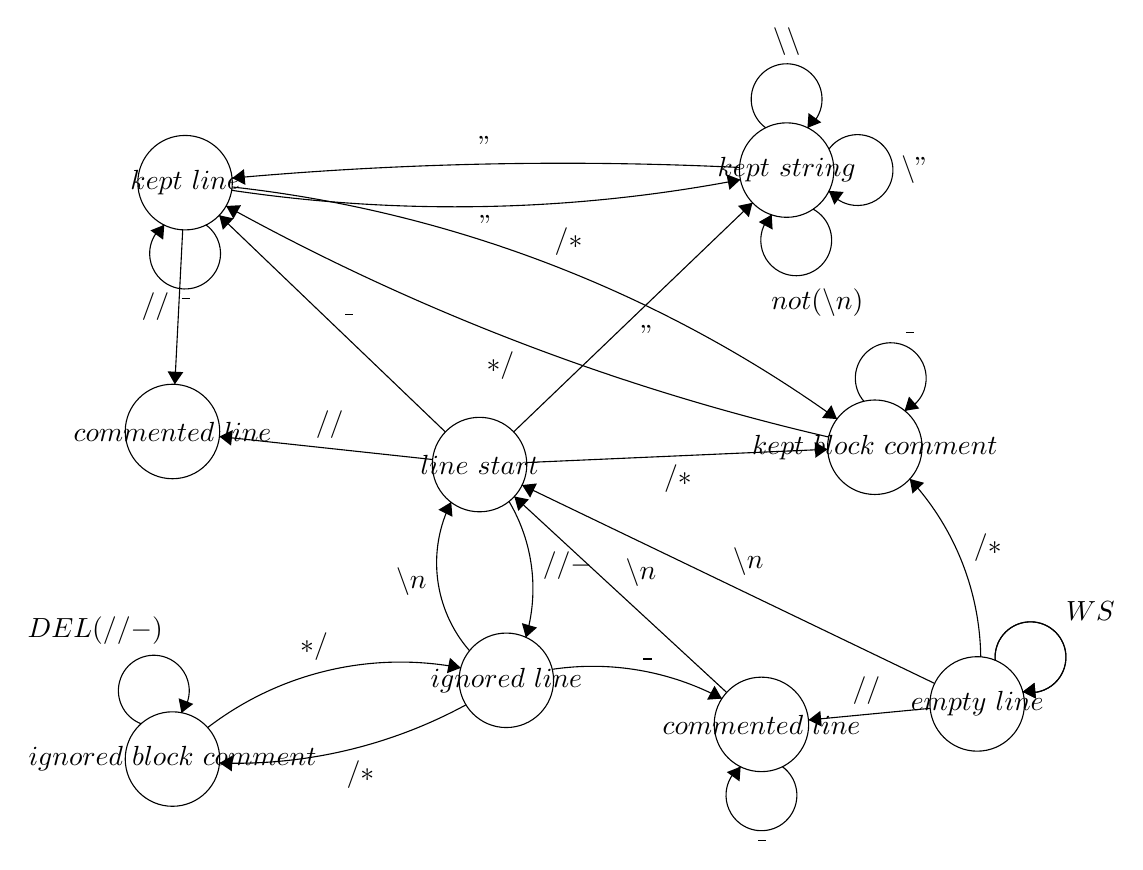
\begin{tikzpicture}[scale=0.2]
\tikzstyle{every node}+=[inner sep=0pt]
\draw [black] (32.6,-29.8) circle (3);
\draw (32.6,-29.8) node {$line\mbox{ }start$};
\draw [black] (34.3,-43.5) circle (3);
\draw (34.3,-43.5) node {$ignored\mbox{ }line$};
\draw [black] (13.1,-27.7) circle (3);
\draw (13.1,-27.7) node {$commented\mbox{ }line$};
\draw [black] (13.9,-11.9) circle (3);
\draw (13.9,-11.9) node {$kept\mbox{ }line$};
\draw [black] (52.1,-11.1) circle (3);
\draw (52.1,-11.1) node {$kept\mbox{ }string$};
\draw [black] (50.5,-46.3) circle (3);
\draw (50.5,-46.3) node {$commented\mbox{ }line$};
\draw [black] (13.1,-48.5) circle (3);
\draw (13.1,-48.5) node {$ignored\mbox{ }block\mbox{ }comment$};
\draw [black] (64.2,-45) circle (3);
\draw (64.2,-45) node {$empty\mbox{ }line$};
\draw [black] (57.7,-28.7) circle (3);
\draw (57.7,-28.7) node {$kept\mbox{ }block\mbox{ }comment$};
\draw [black] (34.467,-32.136) arc (30.72442:-16.57734:10.855);
\fill [black] (35.54,-40.78) -- (36.25,-40.15) -- (35.29,-39.87);
\draw (36.58,-36.21) node [right] {$//-$};
\draw [black] (29.62,-29.48) -- (16.08,-28.02);
\fill [black] (16.08,-28.02) -- (16.82,-28.6) -- (16.93,-27.61);
\draw (23.08,-28.16) node [above] {$//$};
\draw [black] (34.77,-27.72) -- (49.93,-13.18);
\fill [black] (49.93,-13.18) -- (49.01,-13.37) -- (49.7,-14.09);
\draw (43.28,-20.93) node [below] {$"$};
\draw [black] (30.43,-27.73) -- (16.07,-13.97);
\fill [black] (16.07,-13.97) -- (16.3,-14.89) -- (16.99,-14.17);
\draw (24.27,-20.37) node [above] {$\_$};
\draw [black] (13.75,-14.9) -- (13.25,-24.7);
\fill [black] (13.25,-24.7) -- (13.79,-23.93) -- (12.79,-23.88);
\draw (12.93,-19.78) node [left] {$//$};
\draw [black] (49.163,-11.711) arc (-79.13969:-98.46084:96.269);
\fill [black] (49.16,-11.71) -- (48.28,-11.37) -- (48.47,-12.35);
\draw (33.05,-13.93) node [below] {$"$};
\draw [black] (15.223,-14.58) arc (54:-234:2.25);
\draw (13.9,-19.15) node [below] {$\_$};
\fill [black] (12.58,-14.58) -- (11.7,-14.93) -- (12.51,-15.52);
\draw [black] (35.6,-29.67) -- (54.7,-28.83);
\fill [black] (54.7,-28.83) -- (53.88,-28.37) -- (53.93,-29.37);
\draw (45.2,-29.8) node [below] {$/*$};
\draw [black] (16.887,-12.173) arc (83.71258:54.31763:81.07);
\fill [black] (55.3,-26.91) -- (54.94,-26.03) -- (54.35,-26.84);
\draw (38.25,-16.54) node [above] {$/*$};
\draw [black] (57.014,-25.792) arc (221.00538:-66.99462:2.25);
\draw (59.88,-21.55) node [above] {$\_$};
\fill [black] (59.59,-26.39) -- (60.52,-26.24) -- (59.87,-25.48);
\draw [black] (54.771,-28.052) arc (-103.04429:-118.92551:148.313);
\fill [black] (16.51,-13.38) -- (16.97,-14.2) -- (17.45,-13.33);
\draw (33.92,-22.57) node [below] {$*/$};
\draw [black] (16.886,-11.611) arc (95.15989:87.23958:233.306);
\fill [black] (16.89,-11.61) -- (17.73,-12.04) -- (17.64,-11.04);
\draw (32.98,-10.2) node [above] {$"$};
\draw [black] (50.777,-8.42) arc (234:-54:2.25);
\draw (52.1,-3.85) node [above] {${\setminus{}}{\setminus{}}$};
\fill [black] (53.42,-8.42) -- (54.3,-8.07) -- (53.49,-7.48);
\draw [black] (54.78,-9.777) arc (144:-144:2.25);
\draw (59.35,-11.1) node [right] {${\setminus{}}"$};
\fill [black] (54.78,-12.42) -- (55.13,-13.3) -- (55.72,-12.49);
\draw [black] (53.772,-13.576) arc (61.76517:-226.23483:2.25);
\draw (54.05,-18.59) node [below] {$not({\setminus{}}n)$};
\fill [black] (51.15,-13.93) -- (50.33,-14.4) -- (51.21,-14.88);
\draw [black] (31.972,-41.632) arc (-138.85121:-207.00172:8.5);
\fill [black] (30.8,-32.18) -- (29.99,-32.67) -- (30.88,-33.12);
\draw (29.27,-37.22) node [left] {${\setminus{}}n$};
\draw [black] (37.214,-42.802) arc (98.52659:61.86122:17.383);
\fill [black] (47.99,-44.66) -- (47.52,-43.85) -- (47.05,-44.73);
\draw (43.21,-42.27) node [above] {$\_$};
\draw [black] (31.738,-45.058) arc (-61.50966:-91.94905:30.623);
\fill [black] (16.09,-48.75) -- (16.87,-49.28) -- (16.91,-48.28);
\draw (25.03,-48.55) node [below] {$/*$};
\draw [black] (48.29,-44.27) -- (34.81,-31.83);
\fill [black] (34.81,-31.83) -- (35.06,-32.74) -- (35.73,-32.01);
\draw (42.85,-37.56) node [above] {${\setminus{}}n$};
\draw [black] (51.823,-48.98) arc (54:-234:2.25);
\draw (50.5,-53.55) node [below] {$\_$};
\fill [black] (49.18,-48.98) -- (48.3,-49.33) -- (49.11,-49.92);
\draw [black] (15.334,-46.502) arc (127.53688:79.00441:20.093);
\fill [black] (31.41,-42.71) -- (30.72,-42.07) -- (30.53,-43.05);
\draw (22.09,-42.28) node [above] {$*/$};
\draw [black] (11.119,-46.263) arc (249.25512:-38.74488:2.25);
\draw (8.2,-41.25) node [above] {$DEL(//-)$};
\fill [black] (13.67,-45.57) -- (14.42,-45) -- (13.49,-44.64);
\draw [black] (65.346,-42.24) arc (185.18593:-102.81407:2.25);
\draw (69.82,-39.1) node [right] {$WS$};
\fill [black] (67.09,-44.23) -- (67.93,-44.66) -- (67.84,-43.66);
\draw [black] (65.346,-42.24) arc (185.18593:-102.81407:2.25);
\fill [black] (67.09,-44.23) -- (67.93,-44.66) -- (67.84,-43.66);
\draw [black] (59.919,-30.714) arc (42.71431:0.76725:16.992);
\fill [black] (59.92,-30.71) -- (60.09,-31.64) -- (60.83,-30.96);
\draw (63.96,-35.06) node [right] {$/*$};
\draw [black] (61.21,-45.28) -- (53.49,-46.02);
\fill [black] (53.49,-46.02) -- (54.33,-46.44) -- (54.24,-45.44);
\draw (57.17,-45.07) node [above] {$//$};
\draw [black] (61.5,-43.7) -- (35.3,-31.1);
\fill [black] (35.3,-31.1) -- (35.81,-31.9) -- (36.24,-31);
\draw (49.66,-36.89) node [above] {${\setminus{}}n$};
\end{tikzpicture}
\end{center}
\caption{Approximate finite state machine for removing redundant commenting
    from a C file.}\label{fig:comment-simp-fsm}
\end{figure*}

\section{Limitations and future work}

Further input validation on the formatting of fields \emph{within} structs and
unions is also desirable, and should be a relatively straightforward feature to
add.

A useful sanity check on the output of the tree carver is compiling the output
with the same compile command, which should and does not (for the examples we
have used it with so far) produce more warnings than the input code. It would
be even better if the output could be compiled and linked, but this is a
cross-translation-unit issue and the Clang API is fundamentally a
per-translation-unit one, so this requires more consideration and perhaps a
different approach.

Another limitation is that right now, struct fields are omitted with no
replacement, which changes their size. This should be possible to remedy, since
the size and padding of a field are available when traversing the declaration
of a struct field, but leads to a more complex `marking' scheme per line than
the binary included or not. It may also complicate any attempts to link the
code with other code that uses the same struct definitions but different
fields.

\chapter{pKVM Buddy Allocator update}\label{chap:buddy}

\chapter{User experience}

\section{Calling conventions and specifications}

\section{Accurate source location}

Preprocessor column info!

\section{Rich regression testing}

\section{Peformance benchmarking}

\section{Switchable major transitions}

\section{Examples and overfitting}

\section{Updating proofs}

\section{Syntax, syntax, syntax}

\section{Counter examples}\label{sec:counter-ex}

\begin{itemize}
    \item Not minimal
    \item Not consistent
    \item Not easy to relate to source
\end{itemize}

\section{The unreasonable effectiveness of good error messages}\label{sec:error-msgs}

\begin{itemize}
    \item Translate standards jargon into C programmer friendly words.
\end{itemize}

\section{Partnering with industry}

